% ============================================================
% ECON 308 — International Economic Relations
% Lecture 3: Specific Factors and Income Distribution
%            (Chapter 4)
% Fall 2026  |  Muhebullah Karimzada  |  UNBC
% ============================================================
\documentclass[aspectratio=169]{beamer}
\usepackage[utf8]{inputenc}
\usepackage[T1]{fontenc}
\usepackage{lmodern}
\usepackage{textcomp}

%% ── Theme and colours ───────────────────────────────────────
\usetheme{Madrid}
\setbeamertemplate{navigation symbols}{}
\setbeamercovered{transparent}
\setbeamertemplate{itemize items}[circle]
\setbeamertemplate{enumerate items}[default]
\setlength{\parskip}{0.15em}

\definecolor{UNBCDark}    {RGB}{0,74,37}
\definecolor{UNBCGold}    {RGB}{189,155,96}
\definecolor{SoftGray}    {RGB}{244,246,248}
\definecolor{AccentRed}   {RGB}{192,57,43}
\definecolor{AccentBlue}  {RGB}{41,98,255}
\definecolor{AccentTeal}  {RGB}{0,150,136}
\definecolor{AccentOrange}{RGB}{230,126,34}

\setbeamercolor{normal text}         {fg=black,bg=white}
\setbeamercolor{structure}           {fg=UNBCDark}
\setbeamercolor{title}               {fg=white,bg=UNBCDark}
\setbeamercolor{subtitle}            {fg=UNBCGold}
\setbeamercolor{frametitle}          {fg=white,bg=UNBCDark}
\setbeamercolor{block title}         {fg=white,bg=UNBCDark}
\setbeamercolor{block body}          {fg=black,bg=SoftGray}
\setbeamercolor{block title alerted} {fg=white,bg=AccentRed}
\setbeamercolor{block body alerted}  {fg=black,bg=SoftGray}
\setbeamercolor{item}                {fg=UNBCDark}
\setbeamercolor{alerted text}        {fg=AccentRed}
\setbeamercolor{author in head/foot} {fg=white,bg=UNBCDark}
\setbeamercolor{date in head/foot}   {fg=white,bg=UNBCDark}

%% ── Packages ────────────────────────────────────────────────
\usepackage{booktabs,multirow,array,amsmath,amssymb,bm,
            graphicx,adjustbox,tikz,pgfplots,tcolorbox,hyperref}
\tcbuselibrary{skins}
\pgfplotsset{compat=1.18}
\usetikzlibrary{arrows.meta,positioning,calc,shapes.geometric}
\hypersetup{colorlinks=true,linkcolor=UNBCDark}

%% ── Footline ────────────────────────────────────────────────
\setbeamertemplate{headline}{}
\setbeamertemplate{footline}{%
  \leavevmode\hbox{%
  \begin{beamercolorbox}[wd=.78\paperwidth,ht=2.6ex,dp=1.0ex,
                         leftskip=1em]{author in head/foot}%
    \color{white}\textbf{ECON 308}\hspace{0.4em}%
    \textcolor{UNBCGold}{$\vert$}\hspace{0.4em}%
    International Economic Relations%
  \end{beamercolorbox}%
  \begin{beamercolorbox}[wd=.22\paperwidth,ht=2.6ex,dp=1.0ex,
                         rightskip=1em plus 1fil]{date in head/foot}%
    \color{white}\hfill\insertframenumber/\inserttotalframenumber%
  \end{beamercolorbox}}%
}

%% ── Custom tcolorboxes ──────────────────────────────────────
\newtcolorbox{insight}[1]{%
  colback=UNBCGold!12,colframe=UNBCGold!70!black,
  title={\small\bfseries #1},
  left=1mm,right=1mm,top=0.4mm,bottom=0.4mm,
  boxrule=0.5pt,arc=2mm}
\newtcolorbox{canadex}[1][Canadian Example]{%
  colback=AccentTeal!9,colframe=AccentTeal,
  title={\small\bfseries #1},
  left=1mm,right=1mm,top=0.4mm,bottom=0.4mm,
  boxrule=0.5pt,arc=2mm}
\newtcolorbox{discuss}{%
  colback=AccentBlue!8,colframe=AccentBlue,
  title={\small\bfseries Discussion},
  left=1mm,right=1mm,top=0.4mm,bottom=0.4mm,
  boxrule=0.5pt,arc=2mm}
\newtcolorbox{worked}{%
  colback=AccentOrange!8,colframe=AccentOrange,
  title={\small\bfseries Worked Example},
  left=1mm,right=1mm,top=0.4mm,bottom=0.4mm,
  boxrule=0.5pt,arc=2mm}
\newtcolorbox{varbox}{%
  colback=SoftGray,colframe=UNBCDark!40,
  left=1mm,right=1mm,top=0.4mm,bottom=0.4mm,
  boxrule=0.4pt,arc=2mm}

%% ── Figure helpers (column-width aware) ─────────────────────
\newcommand{\FIG}[1]{%
  \begin{center}%
  \includegraphics[width=\columnwidth,height=0.63\textheight,
                   keepaspectratio]{#1}%
  \end{center}}
\newcommand{\FIGS}[2][0.92]{%
  \begin{center}%
  \includegraphics[width=#1\columnwidth,height=0.63\textheight,
                   keepaspectratio]{#2}%
  \end{center}}

%% ── Metadata ────────────────────────────────────────────────
\title{\textbf{Specific Factors and Income Distribution}}
\subtitle{{\large ECON 308\enspace International Economic
  Relations\enspace\textcolor{UNBCGold}{$|$}\enspace
  Chapter~4}}
\author{Muhebullah Karimzada}
\institute{School of Economics\\
           University of Northern British Columbia}
\date{Fall 2026}

% ============================================================
\begin{document}
% ============================================================

%% ─────────────────────────────────────────────────────────────
%% 1. TITLE
%% ─────────────────────────────────────────────────────────────
\begin{frame}[plain]
\titlepage
\end{frame}

%% ─────────────────────────────────────────────────────────────
%% 2. OPENING PUZZLE
%% ─────────────────────────────────────────────────────────────
\begin{frame}[shrink=8]{Opening Puzzle: Why Do Steelworkers Oppose Free Trade?}
\begin{columns}[T]
\begin{column}{0.57\textwidth}
\begin{itemize}
  \item In 2018, the US imposed a \textbf{25\% tariff on
        Canadian steel}.  Hamilton steelworkers cheered.
        Canadian auto workers groaned.
  \item The Ricardian model says \emph{both} countries gain
        from trade.  So why such fierce political opposition?
  \item The Ricardian model is \textbf{too simple}: it has
        one factor (labour) and no distributional conflict.
  \item This chapter adds \textbf{capital} and \textbf{land}
        --- and suddenly trade creates \emph{real} winners
        and losers.
\end{itemize}
\vspace{0.3em}
\begin{insight}{The Distributional Question}
\small Trade raises national income but the gains are not
shared equally.  The Specific Factors Model explains
\emph{who} gains and \emph{who} loses --- and why they
lobby so differently.
\end{insight}
\end{column}
\begin{column}{0.40\textwidth}
\begin{varbox}
\small\textbf{From Ricardo to Reality}\\[0.3em]
\textbf{Ricardian model}: one factor.\\
Everyone gains.  No distributional conflict.\\[0.3em]
\textbf{Specific Factors model}: three factors.\\
Capital and land are \emph{sector-specific} in the
short run.  Trade \textbf{hurts} owners of capital
in the import-competing sector.\\[0.3em]
This is why the political economy of trade is
contentious even when overall welfare rises.
\end{varbox}
\end{column}
\end{columns}
\end{frame}

%% ─────────────────────────────────────────────────────────────
%% 3. WHERE WE ARE
%% ─────────────────────────────────────────────────────────────
\begin{frame}{Where We Are in the Course}
\begin{columns}[T]
\begin{column}{0.55\textwidth}
\begin{itemize}\small
  \item \textbf{Ch.~2} (Lecture~1): Trade facts and the
        gravity model.
  \item \textbf{Ch.~3} (Lecture~2): \emph{Why} trade?
        Comparative advantage; all gain (Ricardian).
  \item \textbf{Ch.~4} (today): \emph{Who gains and who
        loses?}  Short-run specificity of capital and land.
  \item \textbf{Ch.~5} (next): Long-run~--- both factors
        mobile.  H-O model; factor price equalisation.
\end{itemize}
\vspace{0.4em}
\begin{varbox}
\footnotesize\textbf{The two-step logic:}\\[0.2em]
The Specific Factors model is the \emph{short-run} version
of the Heckscher-Ohlin model.  As capital and land become
mobile (long run), SF converges to H-O.\\[0.2em]
\textbf{Ch.~4 = short run;  Ch.~5 = long run.}
\end{varbox}
\end{column}
\begin{column}{0.42\textwidth}
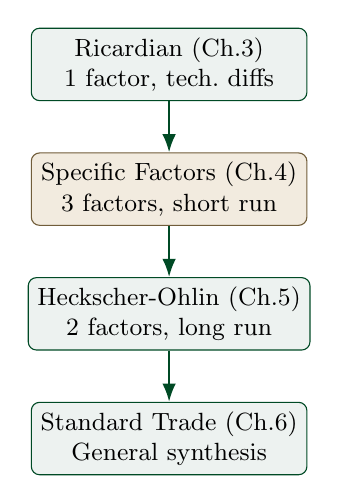
\begin{tikzpicture}[node distance=0.65cm,
  box/.style={draw=UNBCDark,fill=UNBCDark!7,rounded corners=3pt,
              minimum width=3.5cm,minimum height=0.65cm,
              align=center,font=\small}]
  \node[box] (R){Ricardian (Ch.3)\\1 factor, tech.\ diffs};
  \node[box,below=of R,fill=UNBCGold!20,draw=UNBCGold!60!black]
        (SF){Specific Factors (Ch.4)\\3 factors, short run};
  \node[box,below=of SF](HO){Heckscher-Ohlin (Ch.5)\\2 factors, long run};
  \node[box,below=of HO](ST){Standard Trade (Ch.6)\\General synthesis};
  \draw[-{Latex},UNBCDark,thick](R)--(SF);
  \draw[-{Latex},UNBCDark,thick](SF)--(HO);
  \draw[-{Latex},UNBCDark,thick](HO)--(ST);
\end{tikzpicture}
\end{column}
\end{columns}
\end{frame}

%% ─────────────────────────────────────────────────────────────
%% 4. LEARNING OBJECTIVES
%% ─────────────────────────────────────────────────────────────
\begin{frame}{Learning Objectives}
After this lecture you will be able to:
\begin{enumerate}\small
  \item State the assumptions of the specific factors model;
        explain what ``specific'' means and why it matters.
  \item Derive $MPL_M$ and $MPL_F$ and write the labour
        market equilibrium condition.
  \item Solve analytically for the equilibrium wage and
        labour allocation given production functions, prices,
        and endowments.
  \item Predict how a rise in $P_M$ affects wages, capital
        returns, and land returns.
  \item Explain why labour's real wage effect is
        \emph{ambiguous} while specific-factor effects are
        \emph{unambiguous}.
  \item Apply the model to \textbf{Canadian examples}:
        Alberta oil boom, Ontario manufacturing, dairy
        supply management, immigration.
  \item Connect the specific-factors model to the political
        economy of trade protection.
\end{enumerate}
\begin{block}{}
\small Krugman, Obstfeld \& Melitz,
\textit{International Economics}, 12th ed., Chapter~4.
\end{block}
\end{frame}

%% ═══════════════════════════════════════════════════════════
%%  PART 1 — MODEL SETUP
%% ═══════════════════════════════════════════════════════════

%% ─────────────────────────────────────────────────────────────
%% 5. MODEL SETUP
%% ─────────────────────────────────────────────────────────────
\begin{frame}[shrink=5]{Model Setup: Three Factors, Two Sectors}
\begin{columns}[T]
\begin{column}{0.53\textwidth}
\textbf{Two goods:}
\begin{itemize}\small
  \item \textbf{Manufactures (M)}: uses capital $K$ and
        labour $L_M$.
  \item \textbf{Food (F)}: uses land $T$ and labour $L_F$.
\end{itemize}
\vspace{0.3em}
\textbf{Three factors:}
\begin{itemize}\small
  \item \textbf{Labour} $L$:
        \textcolor{AccentTeal}{\textbf{mobile}}~--- moves
        freely between sectors until wages equalise.
  \item \textbf{Capital} $K$:
        \textcolor{AccentRed}{\textbf{specific}} to M only.
  \item \textbf{Land} $T$:
        \textcolor{AccentRed}{\textbf{specific}} to F only.
\end{itemize}
\vspace{0.3em}
\textbf{Why ``specific''?}\\
A steel mill cannot become a wheat farm overnight.
In the short run, capital and land are locked into their
sector.  This is the key departure from the Ricardian
model.
\end{column}
\begin{column}{0.44\textwidth}
\begin{varbox}
\small\textbf{Variable list:}\\[0.2em]
$L=L_M+L_F$ = total labour endowment\\
$K$ = capital (specific to M)\\
$T$ = land (specific to F)\\
$Q_M, Q_F$ = outputs\\
$P_M, P_F$ = goods prices\\
$w$ = wage (equalises across sectors)\\
$r_K = P_M \cdot MPK_M$ = return to capital\\
$r_T = P_F \cdot MPT_F$ = return to land
\end{varbox}
\vspace{0.3em}
\begin{insight}{The Ricardian Bridge}
\footnotesize Ricardian model: 1 factor (labour), linear
PPF, no distributional conflict.\\[0.2em]
Specific Factors: 3 factors, concave PPF,
\emph{some} factors lose from trade.
\end{insight}
\end{column}
\end{columns}
\end{frame}

%% ─────────────────────────────────────────────────────────────
%% 6. PRODUCTION FUNCTIONS AND MPL
%% ─────────────────────────────────────────────────────────────
\begin{frame}[shrink=15]{Production Functions and Marginal Products}
\begin{columns}[T]
\begin{column}{0.53\textwidth}
\textbf{Production functions:}
\[Q_M = F(K,\,L_M), \qquad Q_F = G(T,\,L_F)\]
Both exhibit:
\begin{itemize}\small
  \item \textbf{Positive MPL}: more labour raises output.
  \item \textbf{Diminishing MPL}: each additional unit of
        labour adds less output (holding $K$ or $T$ fixed).
\end{itemize}
\vspace{0.3em}
\textbf{Profit maximisation (competitive equilibrium):}
\[w = P_M\cdot MPL_M(K,L_M) = P_F\cdot MPL_F(T,L_F)\]
Each sector hires labour until the value of its marginal
product equals the wage.\\[0.3em]
These two conditions + $L_M+L_F=L$ determine
$L_M^*$, $L_F^*$, and $w^*$.
\end{column}
\begin{column}{0.44\textwidth}
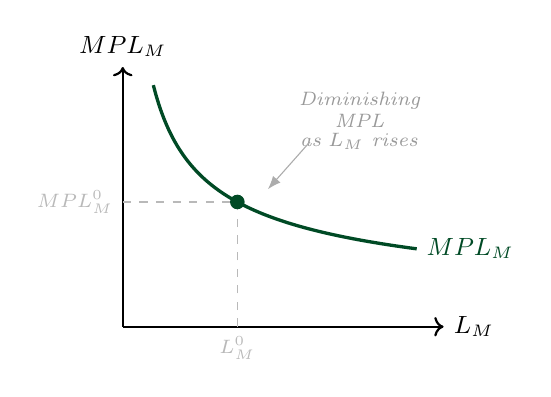
\begin{tikzpicture}[scale=0.97]
  %% Axes
  \draw[->,thick](0,0)--(4.2,0)
       node[right,font=\small]{$L_M$};
  \draw[->,thick](0,0)--(0,3.4)
       node[above,font=\small]{$MPL_M$};
  %% Smooth diminishing MPL: 2.0/sqrt(x)
  %% At x=0.40 → y=3.16 (within chart); at x=3.7 → y=1.04
  \draw[UNBCDark,very thick,domain=0.40:3.85,samples=100]
       plot(\x,{2.0/sqrt(\x)});
  %% Curve label — right end, on the curve
  \node[UNBCDark,font=\small,right] at (3.85,1.02){$MPL_M$};
  %% Reference point at L_M^0=1.5, MPL_M^0≈1.63
  \draw[dashed,gray!55,thin](0,1.633)
       node[left,font=\scriptsize]{$MPL_M^0$} --(1.5,1.633);
  \draw[dashed,gray!55,thin](1.5,0)
       node[below,font=\scriptsize]{$L_M^0$} --(1.5,1.633);
  \filldraw[UNBCDark](1.5,1.633) circle(2.5pt);
  %% Diminishing MPL annotation — upper right, clear of curve
  \node[font=\scriptsize,text=gray!80,text width=2.1cm,
        align=center] at (3.1,2.7)
       {\textit{Diminishing MPL}\\[-1pt]\textit{as $L_M$ rises}};
  \draw[-{Latex},gray!65,thin](2.45,2.42)--(1.90,1.80);
\end{tikzpicture}
\end{column}
\end{columns}
\end{frame}

%% ─────────────────────────────────────────────────────────────
%% 7. THE SF MODEL PPF
%% ─────────────────────────────────────────────────────────────
\begin{frame}[shrink=4]{The Specific Factors PPF: Concave, Not Linear}
\begin{columns}[T]
\begin{column}{0.48\textwidth}
\textbf{Why concave?}
\begin{itemize}\small
  \item When labour shifts from F to M, the first workers
        are highly productive in M (high $MPL_M$) but the
        last workers were still productive in F.
  \item As more labour moves to M, $MPL_M$ falls and the
        lost food output per worker rises.
  \item Each extra unit of M comes at an \emph{increasing}
        OC in terms of F.
\end{itemize}
\vspace{0.3em}
\textbf{Slope} $= -MPL_F/MPL_M = $ opportunity cost of M.\\[0.2em]
As $Q_M$ rises, more labour is in M, so $MPL_M$ falls and
$MPL_F$ rises $\Rightarrow$ slope steepens.\\[0.2em]
\textbf{Contrast with Ricardian}: linear PPF (constant OC).
\end{column}
\begin{column}{0.49\textwidth}
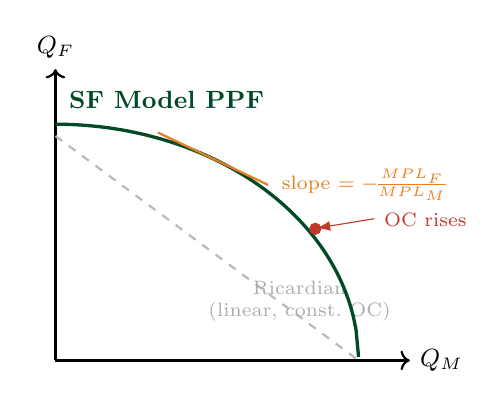
\begin{tikzpicture}[scale=1.0]
  %% Axes
  \draw[->,thick](0,0)--(4.5,0)
       node[right,font=\small]{$Q_M$};
  \draw[->,thick](0,0)--(0,3.7)
       node[above,font=\small]{$Q_F$};
  %% Ricardian PPF: dashed, drawn first (behind)
  \draw[gray!55,thick,dashed](0,2.85)--(3.85,0);
  %% Ricardian label: placed in lower-right clear space
  \node[gray!65,font=\scriptsize,align=center] at (3.1,0.75)
       {Ricardian\\(linear, const.\ OC)};
  %% Concave SF PPF
  \draw[UNBCDark,very thick,domain=0:3.85,samples=120]
       plot(\x,{3.0*sqrt(1-(\x/3.85)^2)});
  %% "SF Model PPF" — upper left, above the curve's starting point
  %% Curve at x=0 is y=3.0; label is at y=3.20 (above curve)
  \node[UNBCDark,font=\small\bfseries,anchor=south west] at (0.05,3.08)
       {\textbf{SF Model PPF}};
  %% Slope tangent at x=2.0: PPF(2.0)=2.562, slope=-0.474
  %% Tangent from (1.3,2.895) to (2.7,2.229)
  \draw[AccentOrange,thick](1.3,2.895)--(2.7,2.229);
  %% Slope label: anchored WEST at right end of tangent (x=2.7)
  %% → starts well right of "SF Model PPF" (which ends at x≈1.6)
  \node[AccentOrange,font=\scriptsize,anchor=west]
       at (2.75,2.23)
       {slope $= -\!\tfrac{MPL_F}{MPL_M}$};
  %% OC rises: dot at lower arc x=3.3, PPF(3.3)=1.672
  \filldraw[AccentRed](3.3,1.672) circle(2pt);
  \draw[-{Latex},AccentRed,thin](4.05,1.8)--(3.32,1.68);
  \node[AccentRed,font=\scriptsize,anchor=west] at (4.05,1.78)
       {OC rises};
\end{tikzpicture}
\end{column}
\end{columns}
\end{frame}

%% ═══════════════════════════════════════════════════════════
%%  PART 2 — LABOUR MARKET EQUILIBRIUM
%% ═══════════════════════════════════════════════════════════

%% ─────────────────────────────────────────────────────────────
%% 8. LABOUR MARKET EQUILIBRIUM: CONCEPT
%% ─────────────────────────────────────────────────────────────
\begin{frame}{Labour Market Equilibrium: The VMPL Diagram}
\begin{columns}[T]
\begin{column}{0.50\textwidth}
\textbf{Equilibrium condition:}
\[P_M\cdot MPL_M = P_F\cdot MPL_F = w\]
\textbf{Reading the diagram:}
\begin{itemize}\small
  \item Horizontal axis: labour in M (left$\to$right) and
        labour in F (right$\to$left); total length $=L$.
  \item $P_M\cdot MPL_M$ slopes \emph{down} as $L_M$
        rises (diminishing MPL in M).
  \item $P_F\cdot MPL_F$ slopes \emph{down} as $L_F$
        rises~--- equivalently, slopes \emph{up} as $L_M$
        rises (reading left to right).
  \item Crossing point: equilibrium $(L_M^*,\,w^*)$.
\end{itemize}
\end{column}
\begin{column}{0.47\textwidth}
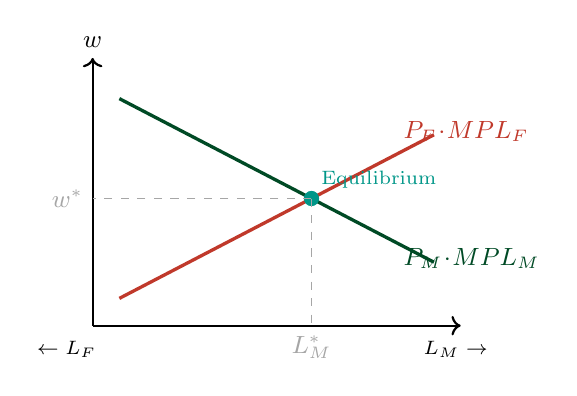
\begin{tikzpicture}[scale=0.85]
  %% Axes
  \draw[->,thick](0,0)--(5.5,0);
  \draw[->,thick](0,0)--(0,4.0) node[above,font=\small]{$w$};
  %% Left-to-right label
  \node[font=\scriptsize,right] at (4.8,-0.35){$L_M\to$};
  \node[font=\scriptsize,left]  at (0.2,-0.35){$\leftarrow L_F$};
  \node[font=\scriptsize,below] at (5.5,0){\phantom{x}};
  %% VMP_M (decreasing in L_M)
  \draw[UNBCDark,very thick,domain=0.4:5.1,samples=50]
       plot(\x,{3.6-0.52*\x});
  \node[UNBCDark,font=\small,right] at (4.5,1.0)
       {$P_M\!\cdot\!MPL_M$};
  %% VMP_F (increasing in L_M = decreasing in L_F)
  \draw[AccentRed,very thick,domain=0.4:5.1,samples=50]
       plot(\x,{0.2+0.52*\x});
  \node[AccentRed,font=\small,right] at (4.5,2.9)
       {$P_F\!\cdot\!MPL_F$};
  %% Equilibrium
  \filldraw[AccentTeal](3.27,1.9) circle(3pt);
  \draw[dashed,gray!70](3.27,1.9)--(3.27,0)
       node[below,font=\small]{$L_M^*$};
  \draw[dashed,gray!70](3.27,1.9)--(0,1.9)
       node[left,font=\small]{$w^*$};
  \node[AccentTeal,font=\scriptsize,above right] at (3.27,1.9)
       {Equilibrium};
\end{tikzpicture}
\end{column}
\end{columns}
\end{frame}

%% ─────────────────────────────────────────────────────────────
%% 9. WORKED EXAMPLE — SETUP
%% ─────────────────────────────────────────────────────────────
\begin{frame}[shrink=20]{Worked Example: Specific Factors with Cobb-Douglas}
\begin{worked}
Home produces Manufactures ($M$) and Food ($F$) with
Cobb-Douglas production:
$Q_M=K^{1/2}L_M^{1/2}$,\quad
$Q_F=T^{1/2}L_F^{1/2}$,\quad
$L_M+L_F=L$.\\[0.2em]
Endowments: $K=144$, $T=64$, $L=100$.
Prices: $P_M=2$, $P_F=1$.
\end{worked}
\vspace{0.3em}
\begin{columns}[T]
\begin{column}{0.50\textwidth}
\textbf{Step 1 — Derive MPLs:}
\[\begin{gathered}
MPL_M = \tfrac{1}{2}K^{1/2}L_M^{-1/2}
       = \dfrac{6}{\sqrt{L_M}}\\[4pt]
MPL_F = \tfrac{1}{2}T^{1/2}L_F^{-1/2}
       = \dfrac{4}{\sqrt{L_F}}
\end{gathered}\]
\textbf{Step 2 — Equalize} ($P_M\!\cdot\!MPL_M = P_F\!\cdot\!MPL_F$):
\[\frac{12}{\sqrt{L_M}} = \frac{4}{\sqrt{100-L_M}}\]
\end{column}
\begin{column}{0.47\textwidth}
\textbf{Step 3 — Solve for $L_M$:}\\[2pt]
Square $\Rightarrow$ $144(100-L_M)=16\,L_M$:
\[14400 = 160\,L_M \;\Rightarrow\;
  \boxed{L_M=90,\; L_F=10}\]
\textbf{Step 4 — Wage:}
\[w = 2\cdot\frac{6}{\sqrt{90}}
    = \frac{12}{\sqrt{90}}
    \approx \mathbf{1.265}\]
\end{column}
\end{columns}
\end{frame}

%% ─────────────────────────────────────────────────────────────
%% 10. WORKED EXAMPLE — VMPL DIAGRAM
%% ─────────────────────────────────────────────────────────────
\begin{frame}[shrink=5]{Worked Example: The VMPL Diagram}
\begin{columns}[T]
\begin{column}{0.44\textwidth}
\textbf{Home's VMPL curves} ($K=144$, $T=64$, $L=100$):
\[\begin{aligned}
w_M(L_M) &= P_M\!\cdot\!MPL_M
           = \frac{12}{\sqrt{L_M}}\\[0.2em]
w_F(L_M) &= P_F\!\cdot\!MPL_F
           = \frac{4}{\sqrt{100-L_M}}
\end{aligned}\]
At $P_M=2$: equilibrium $L_M=90$, $w\approx1.265$.\\[0.3em]
After $P_M$ rises to $3$:
\[w_M' = \frac{18}{\sqrt{L_M}}\]
New equilibrium: $L_M\approx95.2$, $w\approx1.845$.\\[0.3em]
\textbf{Note:} $P_M$ rose by 50\% ($2\to3$) but $w$ rose
only 46\% ($1.265\to1.845$)~--- less than proportionally.
\end{column}
\begin{column}{0.54\textwidth}
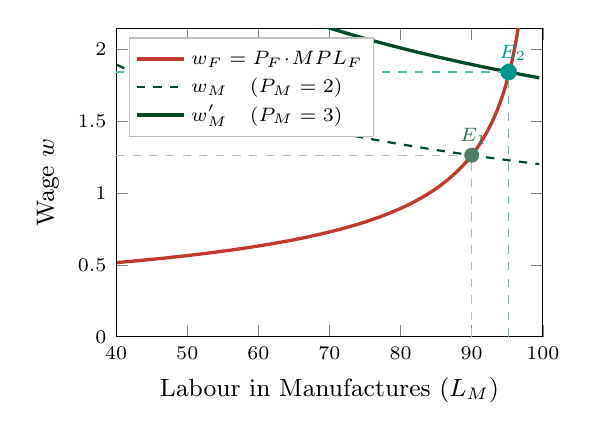
\begin{tikzpicture}
\begin{axis}[
  width=7.0cm, height=5.5cm,
  %% Zoom to region where equilibria are clearly visible
  xmin=40, xmax=100, ymin=0, ymax=2.15,
  xtick={40,50,60,70,80,90,100},
  ytick={0,0.5,1.0,1.5,2.0},
  tick label style={font=\scriptsize},
  xlabel={\small Labour in Manufactures ($L_M$)},
  ylabel={\small Wage~$w$},
  xlabel style={font=\small},
  ylabel style={font=\small},
  legend style={at={(0.03,0.97)},anchor=north west,
                font=\scriptsize,fill=white,
                draw=gray!50,inner sep=2pt,
                row sep=-1pt},
  legend cell align=left,
  clip=true,
  domain=40.1:99.5, samples=300
]
%% Food VMPL: 4/sqrt(100-L_M) — rises steeply near L_M=100
\addplot[AccentRed,very thick]{4/sqrt(100-x)};
\addlegendentry{$w_F = P_F\!\cdot\!MPL_F$\strut}
%% Mfg VMPL (P_M=2): 12/sqrt(L_M) — falls as L_M rises
\addplot[UNBCDark,thick,dashed]{12/sqrt(x)};
\addlegendentry{$w_M$\quad($P_M=2$)\strut}
%% Mfg VMPL (P_M=3): 18/sqrt(L_M) — shifted up
\addplot[UNBCDark,very thick]{18/sqrt(x)};
\addlegendentry{$w_M'$\quad($P_M=3$)\strut}
%% --- Dashed reference lines for E1 (L_M=90, w=1.265) ---
\addplot[dashed,gray!55,thin]
       coordinates{(90,0)(90,1.265)};
\addplot[dashed,gray!55,thin]
       coordinates{(40,1.265)(90,1.265)};
%% --- Dashed reference lines for E2 (L_M=95.2, w=1.845) ---
\addplot[dashed,AccentTeal!65,thin]
       coordinates{(95.2,0)(95.2,1.845)};
\addplot[dashed,AccentTeal!65,thin]
       coordinates{(40,1.845)(95.2,1.845)};
%% --- Equilibrium dots ---
\addplot[mark=*,mark size=2.5pt,only marks,UNBCDark!70]
       coordinates{(90,1.265)};
\addplot[mark=*,mark size=2.8pt,only marks,AccentTeal]
       coordinates{(95.2,1.845)};
%% --- Labels above equilibrium dots ---
\node[font=\scriptsize,anchor=south west,UNBCDark!80]
      at (axis cs:87,1.275){$E_1$};
\node[font=\scriptsize,anchor=south west,AccentTeal]
      at (axis cs:92.5,1.855){$E_2$};
%% --- Axis value labels for equilibria ---
\node[font=\scriptsize,anchor=north,gray!70]
      at (axis cs:90,0){$90$};
\node[font=\scriptsize,anchor=north,gray!70]
      at (axis cs:95.2,0){$95$};
\node[font=\scriptsize,anchor=east,gray!70]
      at (axis cs:40,1.265){$1.27$};
\node[font=\scriptsize,anchor=east,AccentTeal!80]
      at (axis cs:40,1.845){$1.85$};
\end{axis}
\end{tikzpicture}
\end{column}
\end{columns}
\end{frame}

%% ═══════════════════════════════════════════════════════════
%%  PART 3 — PRICE CHANGES AND DISTRIBUTION
%% ═══════════════════════════════════════════════════════════

%% ─────────────────────────────────────────────────────────────
%% 11. EFFECT OF TRADE: P_M RISES
%% ─────────────────────────────────────────────────────────────
\begin{frame}{Effect of Trade: $P_M$ Rises (Home Exports Manufactures)}
\begin{columns}[T]
\begin{column}{0.50\textwidth}
\textbf{Suppose Home's CA is in manufactures.}
Opening to trade raises $P_M$.\\[0.3em]
\textbf{Sequence of effects:}
\begin{enumerate}\small
  \item $P_M\uparrow$ shifts $P_M\cdot MPL_M$ \textbf{up}.
  \item At old wage, M now pays more
        $\Rightarrow$ workers move M $\leftarrow$ F.
  \item $L_M\uparrow$, $L_F\downarrow$.
  \item Wage $w$ rises~--- but \textbf{less than
        proportionally} to $P_M$ (because $MPL_M$ falls
        as more workers crowd into M).
\end{enumerate}
\vspace{0.2em}
\textbf{Key result:}
$\;\hat{w} < \hat{P}_M\;$ (percentage change in wage
is less than percentage change in $P_M$).
\end{column}
\begin{column}{0.47\textwidth}
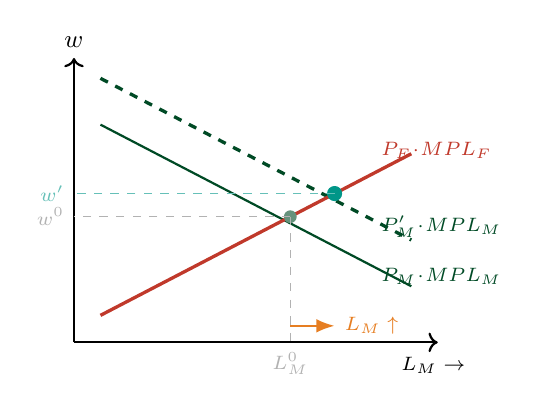
\begin{tikzpicture}[scale=0.84]
  \draw[->,thick](0,0)--(5.5,0);
  \draw[->,thick](0,0)--(0,4.3)
       node[above,font=\small]{$w$};
  \node[font=\scriptsize,right] at (4.8,-0.35){$L_M\to$};
  %% Original VMP_M
  \draw[UNBCDark,thick,domain=0.4:5.1]
       plot(\x,{3.5-0.52*\x});
  \node[UNBCDark,font=\scriptsize,right] at (4.5,1.0)
       {$P_M\!\cdot\!MPL_M$};
  %% Shifted VMP_M
  \draw[UNBCDark,very thick,dashed,domain=0.4:5.1]
       plot(\x,{4.2-0.52*\x});
  \node[UNBCDark,font=\scriptsize,right] at (4.5,1.75)
       {$P_M'\!\cdot\!MPL_M$};
  %% VMP_F
  \draw[AccentRed,very thick,domain=0.4:5.1]
       plot(\x,{0.2+0.52*\x});
  \node[AccentRed,font=\scriptsize,right] at (4.5,2.9)
       {$P_F\!\cdot\!MPL_F$};
  %% Old eq
  \filldraw[UNBCDark!60](3.27,1.9) circle(2.5pt);
  \draw[dashed,gray!60](3.27,1.9)--(0,1.9)
       node[left,font=\scriptsize]{$w^0$};
  \draw[dashed,gray!60](3.27,1.9)--(3.27,0)
       node[below,font=\scriptsize]{$L_M^0$};
  %% New eq
  \filldraw[AccentTeal](3.94,2.25) circle(3pt);
  \draw[dashed,AccentTeal!60](3.94,2.25)--(0,2.25)
       node[left,font=\scriptsize]{$w'$};
  \draw[-{Latex},AccentOrange,thick]
       (3.27,0.25)--(3.94,0.25)
       node[right,font=\scriptsize]{$L_M\uparrow$};
\end{tikzpicture}
\end{column}
\end{columns}
\end{frame}

%% ─────────────────────────────────────────────────────────────
%% 12. WHY LABOUR'S REAL WAGE IS AMBIGUOUS
%% ─────────────────────────────────────────────────────────────
\begin{frame}[shrink=18]{Why Labour's Real Wage Effect is Ambiguous}
\begin{columns}[T]
\begin{column}{0.54\textwidth}
\textbf{Nominal wage rose.  Is labour better off?}\\[0.3em]
After $P_M$ rises: $w$ rose, $P_M$ rose, $P_F$ unchanged.\\[0.3em]
\textbf{Real wage in terms of M} (what matters for
workers who buy manufactures):
\[\frac{w}{P_M} \;\text{ fell}\]
Because $\hat{w} < \hat{P}_M$~--- wage rose less than
the price of manufactures.\\[0.4em]
\textbf{Real wage in terms of F} (what matters for
workers who buy food):
\[\frac{w}{P_F} \;\text{ rose}\]
Because $\hat{w} > 0 = \hat{P}_F$~--- wage rose while
food price is unchanged.
\end{column}
\begin{column}{0.43\textwidth}
\begin{alertblock}{The Ambiguity}
Workers are \textbf{not unambiguously better off} or
worse off~--- it depends on their \textbf{consumption
basket}:\\[0.2em]
\begin{itemize}\small
  \item Workers who mostly \emph{buy goods} (urban
        manufacturing workers): real wage fell in M
        terms~--- \textbf{worse off}.
  \item Workers who mostly \emph{eat} (agricultural
        workers): real wage rose in F terms~---
        \textbf{better off}.
\end{itemize}
\end{alertblock}
\vspace{0.3em}
\begin{insight}{The General Rule}
\footnotesize Labour is the \emph{swing} factor: it
gains in terms of the good whose price \emph{did not}
rise, and loses in terms of the good whose price rose.
\end{insight}
\end{column}
\end{columns}
\end{frame}

%% ─────────────────────────────────────────────────────────────
%% 13. WINNERS AND LOSERS
%% ─────────────────────────────────────────────────────────────
\begin{frame}{Winners and Losers: Unambiguous Factor Returns}
\begin{columns}[T]
\begin{column}{0.52\textwidth}
\begin{block}{Capital owners (specific to M) --- WIN}
\small$r_K = P_M\cdot MPK_M$\\
$P_M\uparrow$ directly boosts revenue.\\
Extra labour flows into M $\Rightarrow$ $MPK_M\uparrow$.\\
\textbf{Double gain: real return to capital rises
unambiguously.}
\end{block}
\vspace{0.3em}
\begin{block}{Landowners (specific to F) --- LOSE}
\small$r_T = P_F\cdot MPT_F$\\
Labour \emph{left} food sector $\Rightarrow$
$L_F\downarrow\Rightarrow MPT_F\downarrow$.\\
$P_F$ unchanged.\\
\textbf{Double loss: real return to land falls
unambiguously.}
\end{block}
\end{column}
\begin{column}{0.45\textwidth}
\begin{alertblock}{Labour --- AMBIGUOUS}
\small Wage $w$ rises, but less than $P_M$ rises.
\begin{itemize}\small
  \item $w/P_M$ falls (lost real purchasing power for
        manufactures).
  \item $w/P_F$ rises (gained real purchasing power for
        food).
\end{itemize}
Net effect depends on the consumption basket.
\end{alertblock}
\vspace{0.3em}
\begin{varbox}
\footnotesize\textbf{Symmetric case ($P_F\uparrow$):}\\
Land owners gain unambiguously.\\
Capital owners lose unambiguously.\\
Labour: ambiguous.
\end{varbox}
\end{column}
\end{columns}
\end{frame}

%% ─────────────────────────────────────────────────────────────
%% 14. SUMMARY TABLE
%% ─────────────────────────────────────────────────────────────
\begin{frame}{Summary: Winners and Losers}
\begin{center}
\begin{adjustbox}{max width=0.95\textwidth}
\begin{tabular}{lllll}
\toprule
\textbf{Factor} & \textbf{Sector} &
\textbf{Effect of $P_M\uparrow$} &
\textbf{Reason} &
\textbf{Trade stance}\\
\midrule
Capital ($K$) & M (export) &
\textcolor{AccentTeal}{\textbf{Gain}} &
Direct $P_M$ gain $+$ more labour in M &
Favour free trade\\
Land ($T$) & F (import-comp.) &
\textcolor{AccentRed}{\textbf{Lose}} &
Labour left F; $MPT_F\downarrow$ &
Oppose free trade\\
Labour ($L$) & Both &
\textit{Ambiguous} &
$w/P_M\downarrow$;\enspace $w/P_F\uparrow$ &
Divided\\
\bottomrule
\end{tabular}
\end{adjustbox}
\end{center}
\vspace{0.3em}
\begin{columns}[T]
\begin{column}{0.52\textwidth}
\begin{insight}{Political Economy Implication}
\small Trade policy is contested because it creates
\textbf{concentrated gains} for some and
\textbf{concentrated losses} for others.\\[0.2em]
Capital owners in export sectors lobby \emph{for}
free trade; specific-factor owners in import-competing
sectors lobby \emph{against} it.
\end{insight}
\end{column}
\begin{column}{0.45\textwidth}
\begin{varbox}
\footnotesize\textbf{Why political opposition persists:}\\[0.2em]
Gains are diffuse (many consumers, each gains a
little).  Losses are concentrated (few capital/land
owners in import-competing sectors, each loses a lot).\\[0.1em]
Concentrated losers lobby harder.
\end{varbox}
\end{column}
\end{columns}
\end{frame}

%% ─────────────────────────────────────────────────────────────
%% 15. THE MAGNIFICATION EFFECT
%% ─────────────────────────────────────────────────────────────
\begin{frame}{The Magnification Effect (Jones, 1971)}
\begin{columns}[T]
\begin{column}{0.53\textwidth}
\begin{block}{Magnification Effect}
If $P_M$ rises by $x\%$ and $P_F$ is unchanged:
\[\hat{r}_K > \hat{P}_M > \hat{w} > \hat{P}_F
  > \hat{r}_T\]
Factor returns change by \emph{more} than goods prices.
\end{block}
\vspace{0.3em}
\textbf{Why?  Capital gets a double gain:}
\begin{enumerate}\small
  \item \emph{Direct}: $P_M$ rises.
  \item \emph{Indirect}: More labour in M
        $\Rightarrow$ $MPK_M\uparrow$.
\end{enumerate}
\textbf{Land suffers a double loss:}
\begin{enumerate}\small
  \item \emph{No direct gain}: $P_F$ unchanged.
  \item \emph{Indirect}: Labour left F
        $\Rightarrow$ $MPT_F\downarrow$.
\end{enumerate}
\end{column}
\begin{column}{0.44\textwidth}
\begin{canadex}[Alberta Oil Boom 2002--2014]
\footnotesize When oil prices tripled, the SF model
predicts:
\vspace{0.2em}
\begin{adjustbox}{max width=\columnwidth}
\begin{tabular}{lc}
\toprule
\textbf{Factor} & \textbf{Effect}\\
\midrule
Oil capital owners & Enormous gains\\
Alberta workers & Wage rise ($+30$--$40\%$)\\
BC/ON manufacturers & Lost workers; costs $\uparrow$\\
Farmers (land) & Hurt (workers left)\\
\bottomrule
\end{tabular}
\end{adjustbox}
\vspace{0.2em}
Magnification: oil capital gains $>$ oil price gain;
manufacturer capital loses $>$ it lost any direct
revenue.
\end{canadex}
\end{column}
\end{columns}
\end{frame}

%% ─────────────────────────────────────────────────────────────
%% 16. DOES THE COUNTRY GAIN OVERALL?
%% ─────────────────────────────────────────────────────────────
\begin{frame}[shrink=5]{Does the Country Gain Overall?}
\begin{columns}[T]
\begin{column}{0.55\textwidth}
\textbf{The aggregate result:}
\begin{itemize}\small
  \item Trade raises \textbf{national income} at world
        prices --- the economy-wide pie grows.
  \item But the gains are \emph{unevenly distributed}:
        export-sector specific factors gain enormously;
        import-sector specific factors lose.
  \item \textbf{Kaldor-Hicks test}: the gainers' gains
        \emph{exceed} the losers' losses, so
        \textbf{compensation is theoretically possible}.
  \item But compensation rarely occurs in practice.
        Trade adjustment assistance programs typically
        cover only a fraction of losses.
\end{itemize}
\end{column}
\begin{column}{0.42\textwidth}
\begin{insight}{The Political Economy Lesson}
\footnotesize Concentrated losses (50,000 steelworkers
losing jobs) are politically visible and generate
intense lobbying.\\[0.2em]
Diffuse gains (38 million consumers each saving
\$200/car) are invisible.\\[0.2em]
This \textbf{asymmetry} explains persistent
protection even when aggregate welfare rises.
\end{insight}
\vspace{0.3em}
\begin{canadex}[CUSMA Dairy Tariffs]
\footnotesize Canadian dairy supply management protects
$\sim$10,000 dairy farmers (specific capital in dairy)
at the expense of 38 million Canadian consumers
paying $\sim$30\% more for dairy products.
\end{canadex}
\end{column}
\end{columns}
\end{frame}

%% ═══════════════════════════════════════════════════════════
%%  PART 4 — CA FROM THE SF MODEL
%% ═══════════════════════════════════════════════════════════

%% ─────────────────────────────────────────────────────────────
%% 17. CA FROM THE SF MODEL
%% ─────────────────────────────────────────────────────────────
\begin{frame}[shrink=5]{Comparative Advantage in the Specific Factors Model}
\begin{columns}[T]
\begin{column}{0.53\textwidth}
\textbf{Opportunity cost of M = slope of PPF:}
\[OC_M = \left.\frac{dQ_F}{dQ_M}\right|_L
        = \frac{MPL_F}{MPL_M}\]
Reallocate $dL$: $dQ_M=MPL_M\,dL_M$,
$dQ_F=-MPL_F\,dL_M$, giving $dQ_F/dQ_M = -MPL_F/MPL_M$.\\[0.3em]
\textbf{With Cobb-Douglas} $Q_M=K^{1/2}L_M^{1/2}$,
$Q_F=T^{1/2}L_F^{1/2}$ (at equal labour split):
\[OC_M = \frac{MPL_F}{MPL_M}
        = \frac{T^{1/2}/\!\sqrt{L/2}}{K^{1/2}/\!\sqrt{L/2}}
        = \frac{T^{1/2}}{K^{1/2}}\]
\textbf{Home} ($K=144$, $T=64$):
$OC_M=\sqrt{64}/\sqrt{144}=8/12=\mathbf{2/3}$.\\
\textbf{Foreign} ($K^*=64$, $T^*=144$):
$OC_M^*=12/8=\mathbf{3/2}$.\\[0.2em]
$2/3<3/2$ $\Rightarrow$ \textbf{Home has CA in M;
Foreign has CA in F.}
\end{column}
\begin{column}{0.44\textwidth}
\begin{insight}{Factor Endowments Determine CA}
\footnotesize Home is \emph{capital-rich} ($K=144>64$)
and \emph{land-poor} ($T=64<144$).\\[0.2em]
Capital-richness lowers the OC of M~---
each unit of M forgoes less F.\\[0.2em]
$\Rightarrow$ Capital-rich countries export
capital-intensive goods (manufactures).\\[0.2em]
$\Rightarrow$ Land-rich countries export
land-intensive goods (food).\\[0.2em]
This is the \textbf{H-O theorem in embryo}:
factor endowments determine comparative advantage.
\end{insight}
\vspace{0.2em}
\begin{varbox}
\footnotesize\textbf{Trade pattern:} At world price
$P_M/P_F\in(2/3,\,3/2)$, Home exports M, Foreign
exports F.
\end{varbox}
\end{column}
\end{columns}
\end{frame}

%% ═══════════════════════════════════════════════════════════
%%  PART 5 — CANADIAN APPLICATIONS
%% ═══════════════════════════════════════════════════════════

%% ─────────────────────────────────────────────────────────────
%% 18. ALBERTA OIL BOOM
%% ─────────────────────────────────────────────────────────────
\begin{frame}{Canadian Application: Alberta Oil Boom}
\begin{columns}[T]
\begin{column}{0.55\textwidth}
\textbf{2002--2014: Global oil demand surged.
Canada's oil exports rose sharply.}\\[0.2em]
\textbf{Mapping to the SF model:}
\begin{itemize}\small
  \item \textbf{Good M}: oil \& gas exports.
  \item \textbf{Good F}: manufactured goods (autos, steel).
  \item \textbf{Capital (K)}: oil sands capital, drilling
        rigs (specific to energy sector).
  \item \textbf{Land (T)}: land and natural resources
        in manufacturing regions (specific to autos/steel).
  \item \textbf{Labour (L)}: mobile workers who moved
        to Fort McMurray.
\end{itemize}
\end{column}
\begin{column}{0.42\textwidth}
\begin{canadex}[SF Model Predictions Confirmed]
\footnotesize\textbf{Winners:}\\
Energy capital owners (\emph{huge} real gains via
magnification).  Alberta wages rose 35--40\%.\\[0.3em]
\textbf{Losers:}\\
Ontario and BC manufacturers lost workers to Alberta
(labour moved west).  Manufacturer capital saw
falling productivity as labour left.\\[0.3em]
\textbf{Labour:}\\
Ambiguous~--- Alberta workers gained; Ontario workers
who stayed faced stagnant wages with rising goods
prices.\\[0.2em]
\textit{This is Dutch Disease: oil boom hurts
manufacturing capital.}
\end{canadex}
\end{column}
\end{columns}
\end{frame}

%% ─────────────────────────────────────────────────────────────
%% 19. ONTARIO MANUFACTURING AND CUSMA
%% ─────────────────────────────────────────────────────────────
\begin{frame}{Canadian Application: Ontario Manufacturing and Trade Shocks}
\begin{columns}[T]
\begin{column}{0.55\textwidth}
\textbf{Two import-competition episodes for Ontario:}\\[0.3em]
\textbf{1. China shock (2001--2015):}
\begin{itemize}\small
  \item Chinese manufactured goods entered Canadian market
        at lower prices.
  \item $P_F$ (import-competing goods) fell~---
        equivalent to adverse $P_F$ shock.
  \item Ontario manufacturing capital (specific) lost
        \emph{unambiguously}.
  \item Workers who stayed in manufacturing saw real
        wage gains (ambiguous channel~--- food prices
        also fell).
\end{itemize}
\vspace{0.2em}
\textbf{2. CUSMA auto content rules:}\\
US tariff threat (2018--20) risked capital loss for
auto-specific capital in Windsor-Oshawa-Oakville.
\end{column}
\begin{column}{0.42\textwidth}
\begin{canadex}[SF Model Lesson for Ontario]
\footnotesize Ontario auto capital is \emph{sector-specific}.
Capital tied to auto assembly cannot quickly pivot to
software or mining.\\[0.2em]
This explains why Ontario auto manufacturers (GM,
Ford, Stellantis) intensely lobbied for CUSMA
protections~--- their specific capital was at risk.\\[0.2em]
\textbf{Policy implication:} Even if overall Canada
gains from CUSMA, sector-specific capital owners in
exposed sectors lose, generating concentrated political
opposition.
\end{canadex}
\end{column}
\end{columns}
\end{frame}

%% ─────────────────────────────────────────────────────────────
%% 20. CANADA'S IMMIGRATION AND THE SF MODEL
%% ─────────────────────────────────────────────────────────────
\begin{frame}{Canadian Application: Immigration as a Labour Supply Shock}
\begin{columns}[T]
\begin{column}{0.53\textwidth}
\textbf{Canada's immigration rate is among the highest
in the OECD}~--- $\sim$400,000 permanent residents/year.\\[0.3em]
\textbf{SF model analysis of a labour supply increase}
($L\uparrow$):
\begin{itemize}\small
  \item Both $L_M$ and $L_F$ absorb more workers.
  \item $MPL_M\downarrow$ and $MPL_F\downarrow$
        $\Rightarrow$ wages fall.
  \item But $MPK_M\uparrow$ (more labour with same $K$)
        $\Rightarrow$ $r_K$ rises.
  \item And $MPT_F\uparrow$ $\Rightarrow$ $r_T$ rises.
  \item \textbf{Capital and land owners gain;
        native workers face wage pressure.}
\end{itemize}
\end{column}
\begin{column}{0.44\textwidth}
\begin{canadex}[Canada's Immigration System]
\footnotesize Canada targets \textbf{skill-complementary}
immigration~--- many arrivals are in healthcare, STEM,
and trades where labour is scarce.\\[0.2em]
\textbf{Key distinction:}
High-skill immigrants \emph{complement} native capital
(raise $MPK$) more than they substitute for native
labour.  Low-skill immigrants compete more directly.\\[0.2em]
\textbf{Net effect in Canada:} capital-intensive sectors
(finance, tech) benefit; wage effects in service/
construction sectors remain contested.
\end{canadex}
\end{column}
\end{columns}
\end{frame}

%% ═══════════════════════════════════════════════════════════
%%  PART 6 — EMPIRICAL EVIDENCE
%% ═══════════════════════════════════════════════════════════

%% ─────────────────────────────────────────────────────────────
%% 21. FIGURE: UNEMPLOYMENT AND IMPORT PENETRATION
%% ─────────────────────────────────────────────────────────────
\begin{frame}[shrink=15]{Evidence: US Unemployment and Import Penetration}
\begin{columns}[T]
\begin{column}{0.52\textwidth}
\FIGS[0.95]{figures/slide46_img01.png}
\end{column}
\begin{column}{0.45\textwidth}
\textbf{What this figure shows:}
\begin{itemize}\small
  \item Horizontal: import penetration ratio
        (imports/domestic consumption) by US industry.
  \item Vertical: unemployment rate in that industry.
  \item Industries with higher import penetration have
        \textbf{higher unemployment}~--- the SF model in
        action.
\end{itemize}
\vspace{0.3em}
\begin{insight}{SF Model Prediction Confirmed}
\footnotesize Workers in import-competing industries
face job losses when trade opens.  This is capital
specificity at work: workers and capital in the wrong
sector cannot instantly redeploy.\\[0.2em]
But \emph{overall} unemployment need not rise~---
workers eventually find other jobs (mobile factor).
\end{insight}
\end{column}
\end{columns}
\end{frame}

%% ─────────────────────────────────────────────────────────────
%% 22. FIGURE: CHINA SHOCK
%% ─────────────────────────────────────────────────────────────
\begin{frame}{Evidence: The China Shock (Autor, Dorn \& Hanson, 2013)}
\begin{columns}[T]
\begin{column}{0.52\textwidth}
\FIGS[0.95]{figures/slide49_img01.png}
\end{column}
\begin{column}{0.45\textwidth}
\textbf{What this figure shows:}
\begin{itemize}\small
  \item US manufacturing employment (left axis) fell
        from $\approx$30\% to $\approx$15\% of the
        workforce, 1960--2020.
  \item Imports from China (right axis) rose from
        $\approx$1\% to $\approx$10\% over the same
        period.
  \item The inverse correlation is striking: as China's
        import share rose, US manufacturing employment
        fell.
\end{itemize}
\vspace{0.2em}
\begin{insight}{SF Model Lesson}
\footnotesize Losses in manufacturing were
\textbf{persistent} (Autor, Dorn \& Hanson, 2013):
workers did not quickly re-employ at similar wages.
This confirms labour is not perfectly mobile in the
short run~--- the SF model's assumption is realistic.
\end{insight}
\end{column}
\end{columns}
\end{frame}

%% ─────────────────────────────────────────────────────────────
%% 23. FIGURE: IMMIGRATION DATA
%% ─────────────────────────────────────────────────────────────
\begin{frame}{Immigration Data: Canada Among Highest in the OECD}
\begin{columns}[T]
\begin{column}{0.52\textwidth}
\FIGS[0.95]{figures/slide60_img01.png}
\end{column}
\begin{column}{0.45\textwidth}
\textbf{What this figure shows:}
\begin{itemize}\small
  \item Foreign-born share of the population across
        selected countries.
  \item \textbf{Switzerland, Australia, Canada}: very
        high (20--30\%).
  \item \textbf{USA}: $\sim$15\% and rising.
\end{itemize}
\vspace{0.3em}
\begin{canadex}[Canada's Immigration Target]
\footnotesize Canada admitted $\sim$405,000 permanent
residents in 2021 and over 400,000 each year
thereafter~--- approximately 1\% of population per
year, among the highest rates in the world.\\[0.2em]
SF model: this labour supply increase \emph{should}
raise returns to Canadian capital and land while
putting downward pressure on wages.
\end{canadex}
\end{column}
\end{columns}
\end{frame}

%% ═══════════════════════════════════════════════════════════
%%  PART 7 — SHORT RUN vs. LONG RUN
%% ═══════════════════════════════════════════════════════════

%% ─────────────────────────────────────────────────────────────
%% 24. SHORT RUN vs. LONG RUN
%% ─────────────────────────────────────────────────────────────
\begin{frame}[shrink=12]{Short Run vs.\ Long Run: Bridge to Chapter 5}
\begin{columns}[T]
\begin{column}{0.53\textwidth}
\begin{adjustbox}{max width=\columnwidth}
\begin{tabular}{lll}
\toprule
\textbf{Feature} & \textbf{Short run (Ch.~4)} &
\textbf{Long run (Ch.~5)}\\
\midrule
Capital & Specific to M & Mobile\\
Land   & Specific to F & Mobile\\
Labour & Mobile & Mobile\\
Factors & 3 ($L$, $K$, $T$) & 2 ($L$, $K$)\\
PPF & Concave (smooth) & Concave (HO)\\
Winners & Clear (specific) & Via Stolper-Sam.\\
\bottomrule
\end{tabular}
\end{adjustbox}
\vspace{0.3em}
\begin{itemize}\small
  \item Short run: a steel mill takes years to redeploy.
        A farm cannot quickly become a factory.
  \item Long run: capital depreciates and re-invests;
        land rezones; factor price equalisation emerges.
  \item Both time horizons matter: workers and capital
        owners care about the short run; economists focus
        on long-run efficiency.
\end{itemize}
\end{column}
\begin{column}{0.44\textwidth}
\begin{insight}{Which Time Horizon Matters?}
\small For policy analysis, both.  Workers and capital
owners in affected sectors care about the \emph{short
run} (their current income and assets).  Policy-makers
focused on long-run efficiency ignore short-run
transitional losses.\\[0.2em]
The political conflict \emph{arises from this mismatch}.
\end{insight}
\vspace{0.3em}
\begin{canadex}[Timeline Analogy]
\footnotesize After NAFTA (1994), Canadian auto parts
manufacturers had perhaps 5--10 years to adjust as
Mexican competition grew.  This transition period
determines whether the SF model or H-O model is more
applicable.
\end{canadex}
\end{column}
\end{columns}
\end{frame}

%% ─────────────────────────────────────────────────────────────
%% 25. MACRO CONNECTIONS
%% ─────────────────────────────────────────────────────────────
\begin{frame}{Macro Connection: Sector-Specific Shocks and the Economy}
\begin{columns}[T]
\begin{column}{0.55\textwidth}
\textbf{The SF model connects to macroeconomics:}
\begin{itemize}\small
  \item \textbf{Commodity boom} (oil price rise):
        energy capital gains, manufacturing capital loses
        $\Rightarrow$ \textbf{Dutch Disease}.
        CAD appreciates, reducing manufactured export
        competitiveness.
  \item \textbf{Regional divergence}: oil boom
        concentrates activity in Alberta; manufacturing
        losses concentrated in Ontario/Quebec.
        Bank of Canada faces a difficult trade-off
        (one interest rate for very different regions).
  \item \textbf{Trade shock $\to$ GDP composition}:
        sector-specific effects change the mix of
        consumption, investment, and exports~---
        affecting aggregate demand and the current
        account.
\end{itemize}
\end{column}
\begin{column}{0.42\textwidth}
\begin{canadex}[SF Model and Bank of Canada]
\footnotesize 2002--2014: Alberta oil boom raised
wages and incomes there but hurt Ontario manufacturing.\\[0.2em]
The Bank of Canada set \emph{one} interest rate for
the whole country.  A rate cut to help Ontario would
overheat Alberta; a rate hike to cool Alberta would
hurt Ontario.\\[0.2em]
This \textbf{regional asymmetry of trade shocks} is
a recurring challenge for Canadian monetary policy~---
rooted in the Specific Factors model.
\end{canadex}
\end{column}
\end{columns}
\end{frame}

%% ─────────────────────────────────────────────────────────────
%% 26. KEY TAKEAWAYS
%% ─────────────────────────────────────────────────────────────
\begin{frame}[shrink=15]{Key Takeaways}
\begin{columns}[T]
\begin{column}{0.57\textwidth}
\begin{enumerate}\small
  \item The SF model has \textbf{three factors}: labour
        (mobile), capital (specific to M), land (specific
        to F).
  \item Equilibrium: $P_M\cdot MPL_M = P_F\cdot MPL_F
        = w$.
  \item A rise in $P_M$ \textbf{unambiguously benefits}
        capital (specific to M) and \textbf{unambiguously
        harms} land (specific to F).
  \item \textbf{Labour is ambiguous}: real wage rises in
        terms of F, falls in terms of M.
  \item \textbf{Magnification effect}: factor returns
        change \emph{more} than goods prices.
  \item Countries gain in aggregate from trade, but
        distribution is unequal~--- political conflict
        is the predictable result.
  \item Canada: Alberta oil capital won, Ontario
        manufacturer capital lost; immigration raises
        capital returns.
  \item \textbf{Short run $\to$ Ch.~4; Long run
        $\to$ Ch.~5}.
\end{enumerate}
\end{column}
\begin{column}{0.40\textwidth}
\begin{block}{Next Lecture: Chapter 5}
\textbf{The Heckscher-Ohlin Model}\\[0.3em]
\small Long run: both capital and labour are mobile
between sectors.\\[0.2em]
Factor endowments (not specific factors) determine
comparative advantage.\\[0.2em]
Factor price equalisation, Stolper-Samuelson theorem,
Rybczynski theorem, Leontief Paradox.
\end{block}
\end{column}
\end{columns}
\end{frame}

%% ─────────────────────────────────────────────────────────────
%% 27. DISCUSSION
%% ─────────────────────────────────────────────────────────────
\begin{frame}[shrink=10]{Discussion Questions}
\begin{columns}[T]
\begin{column}{0.53\textwidth}
\begin{discuss}
\begin{enumerate}\small
  \item In the Canadian forestry sector, who wins and who
        loses when global lumber prices rise?  Map each
        party to the specific factors (capital, land,
        labour).
  \item The US imposed tariffs on Canadian softwood lumber.
        Using the SF model, show \emph{who in the US
        gains} (capital in US forestry) and \emph{who in
        Canada loses} (Canadian forestry capital).
  \item If automation destroys manufacturing jobs, is
        this similar to import competition?  How would
        the SF model describe the distributional effects
        of automation?
  \item Should Canada compensate the losers from trade?
        What policy instruments could achieve this?
\end{enumerate}
\end{discuss}
\end{column}
\begin{column}{0.44\textwidth}
\textbf{Key readings:}
\begin{itemize}\footnotesize
  \item Jones, R.W.\ (1971), ``A Three-Factor Model,''
        \textit{Trade, Balance of Payments and Growth}.
  \item Autor, D., Dorn, D., \& Hanson, G.\ (2013),
        ``The China Syndrome,''
        \textit{American Economic Review}.
  \item Borjas, G.J.\ (1995), ``The Economic Benefits
        from Immigration,''
        \textit{Journal of Economic Perspectives}.
\end{itemize}
\vspace{0.4em}
\begin{block}{Next Lecture}
\small Ch.~5 --- Heckscher-Ohlin: capital and labour,
long-run factor mobility, four major theorems.
\end{block}
\end{column}
\end{columns}
\end{frame}

\end{document}
